% !TeX program = xelatex
\documentclass[12pt,spanish,letterpaper,oneside]{article}
\PassOptionsToPackage{es-noshorthands}{babel}
\def\documenttitle{El sistema de endomembranas como red logística celular}
\def\documentsubtitle{Reporte técnico integrador de tránsito vesicular y clasificación proteica}
\def\documentsubject{Biología Celular --- Ingeniero Agrónomo}
\def\documentauthor{Diego de la Cruz}
\def\coursename{Biología Celular}
\def\coursecode{}
\def\universityname{Universidad Autónoma de Nuevo León}
\def\universityfaculty{Facultad de Agronomía}
\def\universitydepartment{Ingeniero Agrónomo}
\def\universitydepartmentimage{departamentos/logos-institucionales.pdf}
\def\universitydepartmentimagecfg{height=2.1cm}
\def\universitylocation{General Escobedo, Nuevo León, México}
\def\authortable{%
	\begin{Form}
	\begin{tabular}{@{}ll@{}}
		\textbf{Estudiante:} & Diego de la Cruz\\[0.35cm]
		\textbf{Plantel / Sede:} & Campus Escobedo (General Escobedo, N.L.)\\[0.35cm]
		\textbf{Docente Titular:} & Dr. Miguel Ángel Dector Carrillo\\[0.35cm]
		\textbf{Unidad de Aprendizaje:} & Biología Celular\\[0.5cm]
		\multicolumn{2}{l}{Fecha de realización: 18 de octubre de 2026}\\
		\multicolumn{2}{l}{\universitylocation}
	\end{tabular}
	\end{Form}
}

\usepackage{fontspec}
\setmainfont{Arial}
\setsansfont{Arial}
\AddToHook{file/config.tex/after}[aulatex-biologia-celular]{%
  \def\documentfontsize{12}
  \def\documentinterline{1}
  \def\documentparindent{0}
  \def\documentparskip{5}
  \def\fontdocument{custom}
  \def\fonttypewriter{custom}
  \def\stylecitereferences{custom}
  \def\portraitstyle{style1}
  \def\hfstyle{style1}
  \def\hfwidthwrap{true}
  \def\hfwidthtitle{0.44}
  \def\hfwidthcourse{0.52}
  \def\predocpageromannumber{false}
  \def\pagemarginleft{2.5}
  \def\pagemarginright{2.5}
  \def\pagemargintop{2.5}
  \def\pagemarginbottom{2.5}
  \def\firstpagemargintop{3.8}
  \def\sectionfontsize{\large}
  \def\sectionspacingtop{8}
  \def\sectionspacingbottom{4}
  \def\ssectionfontsize{\normalsize}
  \def\ssectionspacingtop{6}
  \def\ssectionspacingbottom{3}
  \def\defaultimagefolder{UANL/ingeniero-agronomo/biologia-celular/img/}
  \def\usepdfmetadata{false}
}
% Template:     Informe LaTeX
% Documento:    Núcleo del template
% Versión:      DEV
% Codificación: UTF-8
%
% Autor: Pablo Pizarro R.
%        pablo@ppizarror.com
%
% Manual template: [https://latex.ppizarror.com/informe]
% Licencia MIT:    [https://opensource.org/licenses/MIT]

% -----------------------------------------------------------------------------
% CONFIGURACIONES
% -----------------------------------------------------------------------------
% Definiciones previas
\input{src/defs}

% Ajustes usuario
\input{src/config}

% -----------------------------------------------------------------------------
% IMPORTACIÓN DE LIBRERÍAS
% -----------------------------------------------------------------------------
\input{src/env/imports}

% -----------------------------------------------------------------------------
% IMPORTACIÓN DE FUNCIONES Y ENTORNOS
% -----------------------------------------------------------------------------
\input{src/cmd/core}
\input{src/cmd/math}
\input{src/cmd/equation}
\input{src/cmd/image}
\input{src/cmd/title}
\input{src/cmd/other}
\input{src/cmd/column}
\input{src/env/environments}

% -----------------------------------------------------------------------------
% IMPORTACIÓN DE ESTILOS
% -----------------------------------------------------------------------------
\input{src/style/code}
\input{src/style/other}

% -----------------------------------------------------------------------------
% CONFIGURACIÓN INICIAL DEL DOCUMENTO
% -----------------------------------------------------------------------------
\input{src/cfg/init}

% -----------------------------------------------------------------------------
% PORTADA
% -----------------------------------------------------------------------------
\input{src/page/portrait}
\input{src/page/portrait_config}

% -----------------------------------------------------------------------------
% CONFIGURACIÓN DE PÁGINA Y ENCABEZADOS
% -----------------------------------------------------------------------------
\input{src/cfg/page}

% -----------------------------------------------------------------------------
% TABLA DE CONTENIDOS - ÍNDICE
% -----------------------------------------------------------------------------
\input{src/page/index}

% -----------------------------------------------------------------------------
% CONFIGURACIONES FINALES
% -----------------------------------------------------------------------------
\input{src/cfg/final}

\RemoveFromHook{file/config.tex/after}[aulatex-biologia-celular]


\usepackage{tabularx}
\usepackage{booktabs}
\usepackage{amsmath,amssymb}
\usepackage{graphicx}
\usepackage{pdflscape}
\usepackage{tikz}
\usetikzlibrary{shapes,arrows.meta,positioning,calc,fit,backgrounds}
\usepackage[backend=biber,style=apa,sorting=nyt]{biblatex}
\definecolor{uanlblue}{RGB}{0,55,108}
\definecolor{tableblue}{RGB}{233,240,247}
\definecolor{proccolor}{RGB}{15,115,55}
\definecolor{protcolor}{RGB}{195,60,10}
\definecolor{pathcolor}{RGB}{110,30,140}
\definecolor{boxbg}{RGB}{246,249,253}
\def\portraittitlecolor{uanlblue}
\def\sectioncolor{uanlblue}
\def\ssectioncolor{uanlblue}
\def\documenttitlehf{Sistema de Endomembranas}
\hypersetup{colorlinks=true,linkcolor=uanlblue,urlcolor=uanlblue,citecolor=uanlblue,pdfauthor={Diego de la Cruz},pdftitle={El sistema de endomembranas como red logística celular},pdfsubject={Sistema de Endomembranas --- Biología Celular UANL}}
\addbibresource{UANL/ingeniero-agronomo/biologia-celular/biologia-celular.bib}
\newcolumntype{Z}{>{\raggedright\arraybackslash}X}
\setlength{\emergencystretch}{2.5em}

\begin{document}
\hypersetup{pageanchor=false}
\begingroup
\fontsize{14}{17}\selectfont
\renewcommand{\Huge}{\fontsize{14}{17}\selectfont\bfseries}
\renewcommand{\large}{\fontsize{14}{17}\selectfont}
\templatePortrait
\clearpage
\endgroup
\hypersetup{pageanchor=true}
\templatePagecfg
\singlespacing
\setlength{\tabcolsep}{6pt}
\renewcommand{\arraystretch}{1.18}

\section*{Resumen}
En este reporte explico el funcionamiento del sistema de endomembranas en la célula eucariota, entendiéndolo como una red de transporte donde se fabrican, modifican y entregan proteínas a sus destinos. Con el ejemplo de la célula acinar pancreática, sigo y comparo el trayecto de dos proteínas: una enzima digestiva (zimógeno) que se almacena y se libera al exterior por secreción regulada, y una hidrolasa ácida que se envía al lisosoma para degradar sustancias de desecho. Reviso cada etapa: el inicio en ribosomas libres, la entrada al retículo endoplásmico rugoso (RER) por el péptido señal y la translocación cotraduccional, la N-glucosilación, el viaje al aparato de Golgi en vesículas COPII, los cambios que sufren los azúcares en las cisternas y la selección final en la red \textit{trans}-Golgi. También respondo cuatro preguntas sobre la función del aparato de Golgi como centro de distribución, por qué el retículo y el Golgi son estaciones de paso, qué pasa cuando falta la señal de manosa-6-fosfato y las diferencias entre las cubiertas COPII, COPI y clatrina, relacionando estos temas con su importancia en la agronomía y los cultivos.

\vspace{0.2cm}
\noindent\textbf{Palabras clave:} Sistema de endomembranas, translocación cotraduccional, red \textit{trans}-Golgi, manosa-6-fosfato, cubiertas vesiculares, secreción regulada, lisosoma.

\section{Introducción y Modelo Biológico Pancreático}
Las células eucariotas están divididas por membranas internas en varios compartimentos u organelos. Esto permite que ocurran diferentes reacciones químicas al mismo tiempo sin que choquen entre sí \parencite{alberts2022molecular}. Estos organelos forman el sistema de endomembranas, una red coordinada que fabrica, procesa y distribuye proteínas y lípidos a donde se necesitan \parencite{lodish2021molecular, fortoul2020histologia}.

Para analizar este proceso, tomo como modelo la célula acinar del páncreas \parencite{kierszenbaum2020histologia}. Esta célula trabaja produciendo dos tipos de proteínas muy diferentes: enzimas digestivas inactivas (como tripsinógeno y amilasa) que almacena para liberarlas solo cuando se digieren alimentos, e hidrolasas ácidas que deben enviarse de forma directa y segura a los lisosomas para reciclar materiales sin destruir a la propia célula \parencite{karp2019biologia, lieberman2018marks}.

\section{Morfología y Componentes del Sistema de Endomembranas}
Para visualizar esta red, en la siguiente página presento el esquema del sistema de endomembranas en formato horizontal (Esquema I / Figura~\ref{fig:esquema_endomembranas}), mostrando cómo se conectan los organelos:

\clearpage
\newgeometry{margin=0.35cm}
\pagestyle{empty}
\begin{landscape}
\thispagestyle{empty}
\refstepcounter{figure}\label{fig:esquema_endomembranas}%
\centering
\noindent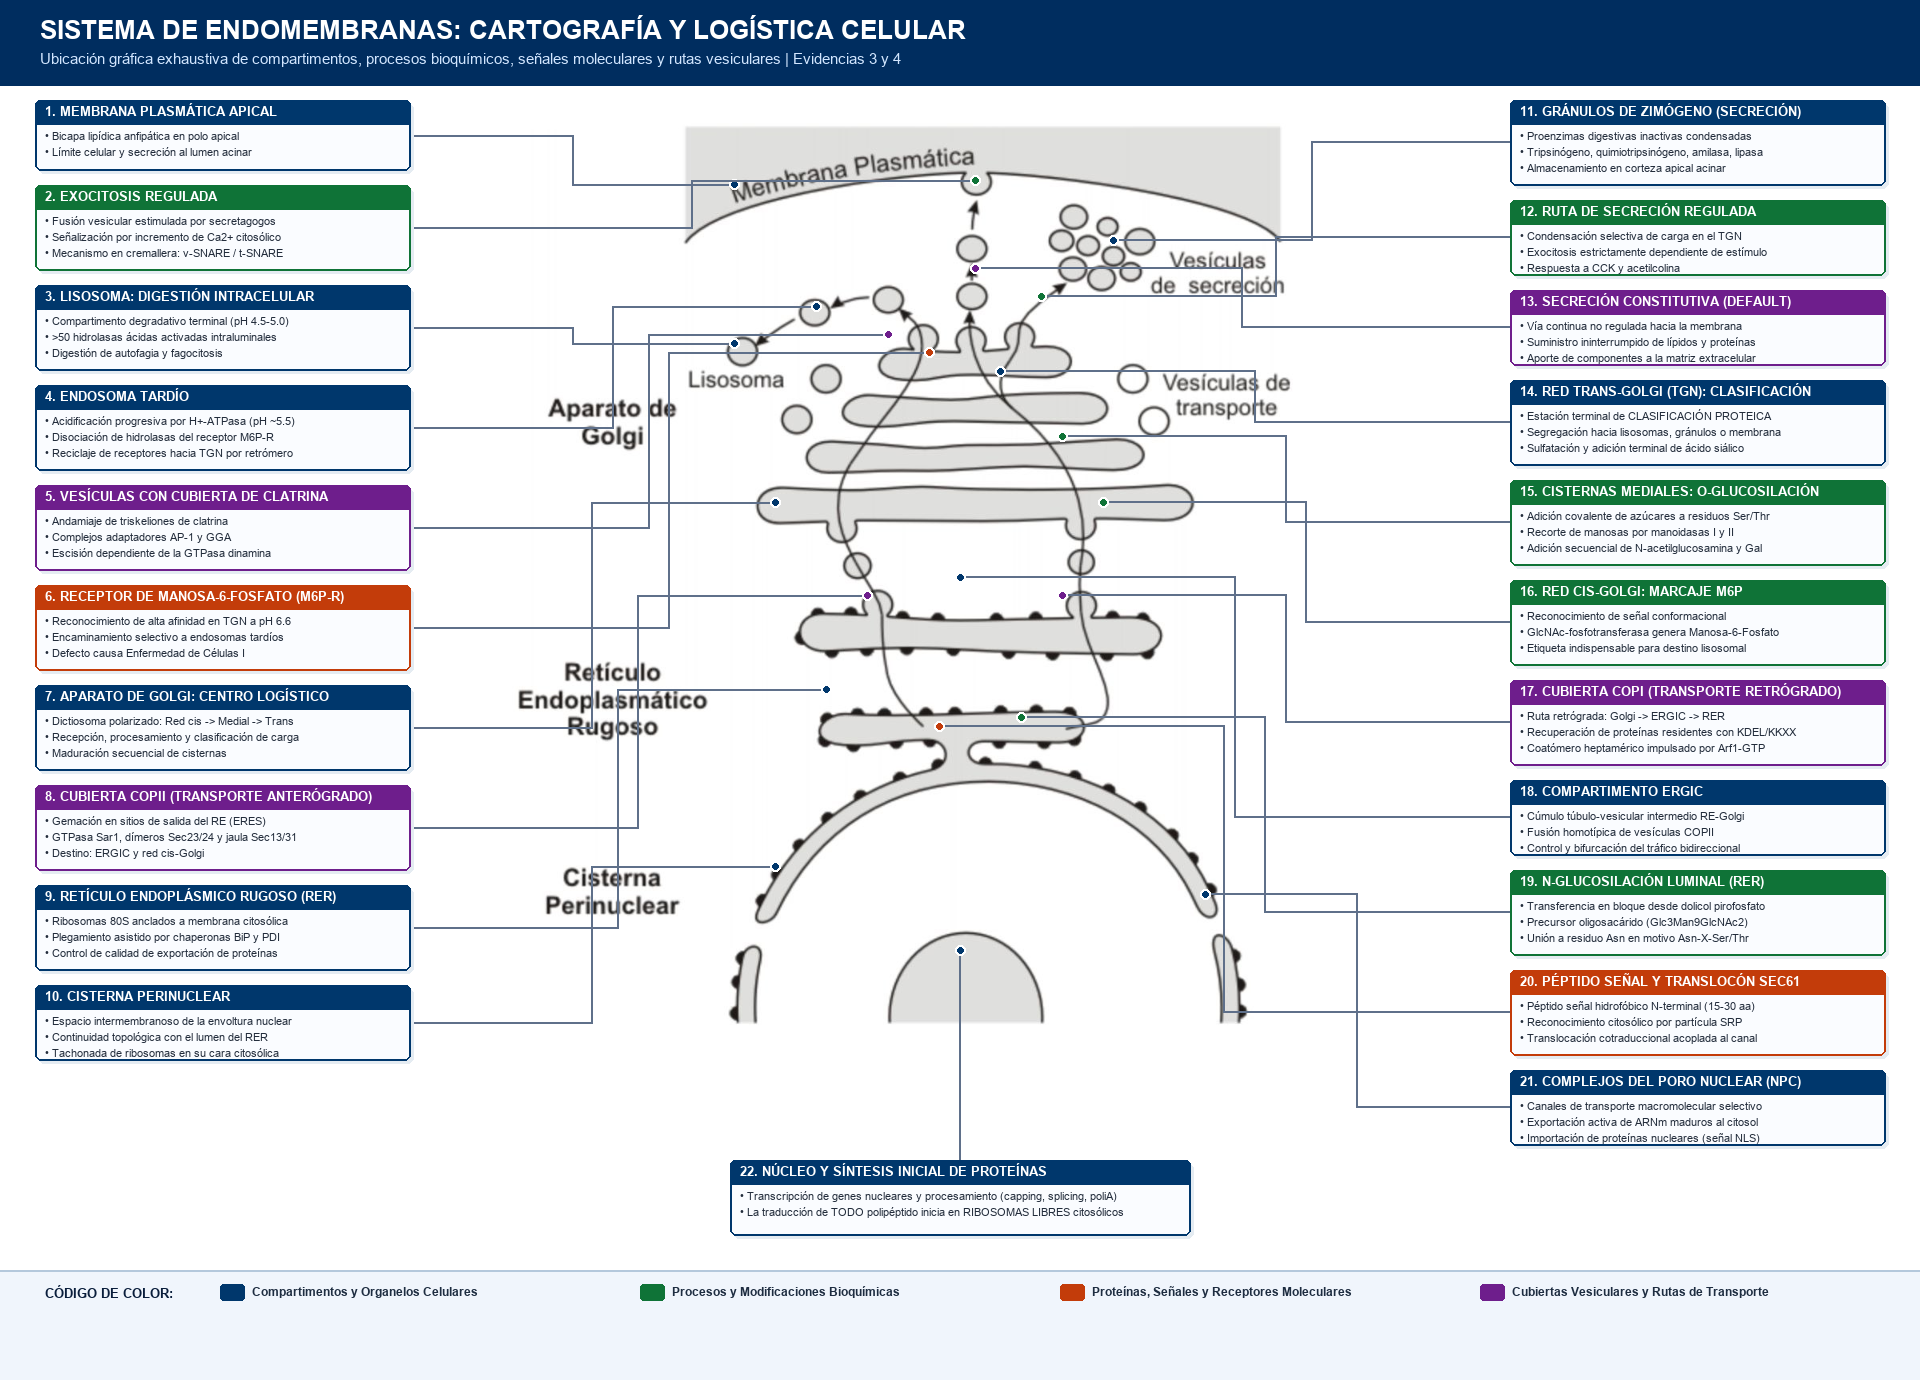
\includegraphics[width=\linewidth,height=\textheight,keepaspectratio]{esquema-endomembranas-anotado.png}
\end{landscape}
\restoregeometry
\clearpage
\pagestyle{fancy}

A partir de este esquema, reviso los compartimentos principales de la red y qué hace cada uno:
\begin{enumerate}
    \item \textbf{Cisterna Perinuclear y Envoltura Nuclear:} Doble membrana que rodea al núcleo y se conecta con el RER. Presenta poros nucleares que permiten la salida del ARN mensajero hacia el citoplasma para su traducción \parencite{fortoul2020histologia}.
    \item \textbf{Retículo Endoplásmico Rugoso (RER):} Sacos membranosos aplanados con ribosomas pegados en su superficie exterior. Es el lugar donde entran las proteínas de secreción o de lisosoma mientras se van sintetizando, donde se pliegan con ayuda de chaperonas y reciben su primera modificación con azúcares (N-glucosilación) \parencite{salazar2018biologia}.
    \item \textbf{Retículo Endoplásmico Liso (REL):} Red de túbulos sin ribosomas, continua con el RER. Se encarga de sintetizar lípidos y fosfolípidos, detoxificar sustancias extrañas y almacenar iones de calcio ($Ca^{2+}$) \parencite{karp2019biologia}.
    \item \textbf{Compartimento Intermedio RE-Golgi (ERGIC):} Grupo de vesículas que se unen al salir del retículo y sirven como primera estación de paso antes de entrar a la cara de entrada del aparato de Golgi \parencite{alberts2022molecular}.
    \item \textbf{Aparato de Golgi:} Conjunto de sacos aplanados y apilados (dictiosoma) que procesa y clasifica proteínas en tres zonas principales:
    \begin{itemize}
        \item \textbf{Red \textit{cis}-Golgi:} Cara de entrada orientada hacia el núcleo y el RER, donde se reciben las vesículas y se coloca la marca de fosfato en las enzimas de lisosoma.
        \item \textbf{Cisternas Mediales:} Región intermedia donde se recortan manosas y se agregan nuevos azúcares a las proteínas, incluyendo la O-glucosilación \parencite{mathews2013bioquimica}.
        \item \textbf{Cara \textit{trans} y Red \textit{trans}-Golgi (TGN):} Cara de salida orientada hacia la membrana celular, donde las proteínas se clasifican y empacan en vesículas específicas según a dónde deben dirigirse \parencite{fortoul2020histologia}.
    \end{itemize}
    \item \textbf{Vesículas de Transporte:} Pequeñas esferas de membrana que transportan proteínas y lípidos de un compartimento a otro dentro de la célula \parencite{lodish2021molecular}.
    \item \textbf{Vesículas de Secreción (Gránulos de Zimógeno):} Vesículas grandes donde se concentran y guardan las enzimas digestivas en espera de una señal para ser liberadas \parencite{kierszenbaum2020histologia}.
    \item \textbf{Endosomas (Tempranos y Tardíos):} Compartimentos con medio ácido que reciben sustancias que entran por endocitosis y participan en el envío de enzimas hacia los lisosomas \parencite{alberts2022molecular}.
    \item \textbf{Lisosomas:} Organelos digestivos de la célula que tienen enzimas que trabajan a pH ácido ($pH \approx 4.5-5.0$) para destruir desechos y reciclar componentes celulares \parencite{fortoul2020histologia, lieberman2018marks}.
    \item \textbf{Membrana Plasmática:} Límite exterior de la célula; aquí se fusionan las vesículas de secreción para vaciar su contenido al exterior mediante exocitosis.
\end{enumerate}

\section{Parte I. Construcción de la Ruta Celular y Encaminamiento Proteico}
Tomando como base la célula del páncreas, explico el camino detallado de las dos proteínas modelo que sintetiza la célula:

\subsection{Ruta 1: Enzima Digestiva de Secreción Regulada (Zimógeno, e.g. Tripsinógeno)}
Sigo primero el recorrido de la enzima digestiva que saldrá al exterior:
\begin{enumerate}
    \item \textbf{Inicio de la síntesis en el citosol:} El gen se transcribe a ARNm en el núcleo, sale al citoplasma por los poros y un \textbf{ribosoma citosólico libre} empieza la traducción.
    \item \textbf{Péptido señal y entrada al RER:} Los primeros 15 a 30 aminoácidos forman el \textbf{péptido señal}. La partícula SRP reconoce esta señal, frena un momento la traducción y guía el ribosoma hacia la membrana del \textbf{RER}. El ribosoma se conecta al canal Sec61 y la proteína va entrando al interior del retículo al mismo tiempo que se fabrica (\textbf{traducción cotraduccional}) \parencite{salazar2018biologia, alberts2022molecular}.
    \item \textbf{Procesamiento inicial en el RER:} Una enzima corta el péptido señal y se le pega un azúcar precursor a un residuo de asparagina (\textbf{N-glucosilación}). Proteínas chaperonas (como BiP y calnexina) ayudan a que la enzima se pliegue de forma correcta \parencite{mathews2013bioquimica}.
    \item \textbf{Viaje hacia el Golgi por COPII:} Las enzimas bien plegadas se empaquetan en vesículas con cubierta \textbf{COPII}. Estas vesículas salen del retículo, pasan por el compartimento intermedio \textbf{ERGIC} y se fusionan con la cara \textit{cis} del aparato de Golgi \parencite{fortoul2020histologia, lodish2021molecular}.
    \item \textbf{Modificación en el Golgi:} La proteína avanza por las cisternas del dictiosoma, donde se le recortan manosas y se le agregan otros azúcares complejos, realizándose la \textbf{O-glucosilación} en residuos de serina o treonina \parencite{mathews2013bioquimica, kierszenbaum2020histologia}.
    \item \textbf{Clasificación en la red trans-Golgi:} Al llegar a la red \textit{trans}-Golgi (\textbf{TGN}), la célula realiza la \textbf{clasificación proteica}. Como la enzima digestiva no tiene marca de lisosoma, se agrupa en vesículas que formarán gránulos para la \textbf{secreción regulada} \parencite{alberts2022molecular}.
    \item \textbf{Almacenamiento y exocitosis:} Los gránulos maduran y quedan guardados en la parte superior de la célula acinar. Cuando llega una señal digestiva que sube los niveles de $Ca^{2+}$, las vesículas se fusionan con la membrana celular y expulsan las enzimas por \textbf{exocitosis} hacia el conducto pancreático \parencite{kierszenbaum2020histologia, karp2019biologia}.
\end{enumerate}

\subsection{Ruta 2: Enzima Lisosomal (Hidrolasa Ácida, e.g. Fosfatasa Ácida / Catepsina)}
A continuación, reviso el camino de una hidrolasa ácida que debe quedarse en los lisosomas:
\begin{enumerate}
    \item \textbf{Inicio y translocación al RER:} Igual que el zimógeno, empieza en ribosomas libres y entra al interior del \textbf{RER} gracias a su \textbf{péptido señal} por \textbf{traducción cotraduccional}.
    \item \textbf{N-glucosilación en el RER:} En el lumen del retículo se corta el péptido señal, la enzima recibe el azúcar precursor por \textbf{N-glucosilación} y se pliega con ayuda de chaperonas.
    \item \textbf{Salida en vesículas COPII:} La prohidrolasa viaja hacia la cara \textit{cis} del Golgi dentro de vesículas con cubierta \textbf{COPII}.
    \item \textbf{La marca de manosa-6-fosfato en el Golgi:} En la red \textit{cis}-Golgi se realiza el marcaje clave para su \textbf{encaminamiento proteico}: una enzima reconoce una zona especial de la hidrolasa y le pega un fosfato a una de sus manosas, produciendo la marca de \textbf{manosa-6-fosfato} (M6P) \parencite{mathews2013bioquimica, alberts2022molecular}.
    \item \textbf{Reconocimiento por el receptor y cubierta de clatrina:} En la red \textit{trans}-Golgi (\textbf{TGN}), el \textbf{receptor de manosa-6-fosfato} (MPR) reconoce esta marca y sujeta a la enzima. Por el lado del citosol, el receptor atrae adaptadores y forma una jaula de \textbf{clatrina}. La vesícula se desprende con ayuda de la proteína dinamina \parencite{lodish2021molecular, fortoul2020histologia}.
    \item \textbf{Entrega al endosoma y reciclaje del receptor:} La vesícula pierde su cubierta de clatrina y se une a un \textbf{endosoma tardío}. Como el interior del endosoma es ácido ($pH \approx 5.5$), la enzima se suelta del receptor. Los receptores vacíos se regresan al TGN para volver a usarse, y a la manosa se le retira el fosfato para evitar que la enzima vuelva a pegarse al receptor \parencite{alberts2022molecular, kierszenbaum2020histologia}.
    \item \textbf{Activación en el lisosoma:} El endosoma madura y se convierte en un \textbf{lisosoma} activo, con un pH de 4.5 a 5.0, donde la enzima empieza a degradar desechos y materiales celulares viejos \parencite{fortoul2020histologia, lieberman2018marks}.
\end{enumerate}

\subsection{Cuadro Comparativo Secuencial del Tránsito de Carga}

\begin{table}[htbp]
\centering
\footnotesize
\begin{tabularx}{\textwidth}{p{3.2cm}ZZ}
\toprule
\textbf{Etapa del Proceso} & \textbf{Proteína 1: Enzima Digestiva (Zimógeno)} & \textbf{Proteína 2: Hidrolasa Lisosomal} \\
\midrule
\textbf{Inicio de Síntesis} & Ribosoma citosólico libre; parada por SRP. & Ribosoma citosólico libre; parada por SRP. \\
\textbf{Mecanismo de Entrada} & Translocación cotraduccional (canal Sec61). & Translocación cotraduccional (canal Sec61). \\
\textbf{Modificación en RER} & N-glucosilación ($Glc_3Man_9GlcNAc_2$), corte de señal. & N-glucosilación ($Glc_3Man_9GlcNAc_2$), corte de señal. \\
\textbf{Tránsito RER $\to$ Golgi} & Vesículas anterógradas con cubierta COPII. & Vesículas anterógradas con cubierta COPII. \\
\textbf{Modificación en Golgi} & O-glucosilación y maduración glicídica compleja. & Adición del marcador manosa-6-fosfato (M6P). \\
\textbf{Clasificación en TGN} & Condensación en agregados insolubles apicales. & Reconocimiento selectivo por receptor MPR. \\
\textbf{Cubierta Post-Golgi} & Sin cubierta de clatrina; gemación de gránulos. & Vesículas recubiertas de triskeliones de clatrina. \\
\textbf{Compartimento Intermedio} & Gránulos de secreción inmaduros apicales. & Endosoma tardío acidificado ($pH \approx 5.5$). \\
\textbf{Mecanismo de Descarga} & Exocitosis regulada estimulada por $Ca^{2+}$. & Maduración endosomal y digestión intraluminal. \\
\textbf{Destino Celular Final} & Exterior celular (lumen del ácino pancreático). & Lisosoma maduro (pH 4.5--5.0). \\
\bottomrule
\end{tabularx}
\caption{Matriz comparativa de tránsito, modificación y destino para las dos proteínas modelo.}
\label{tab:comparativo_rutas}
\end{table}

Para comparar de forma sencilla el camino de ambas proteínas desde que salen del retículo, en la Figura~\ref{fig:esquema_rutas} presento un diagrama de flujo que resume el trayecto de la enzima digestiva y de la hidrolasa lisosomal:

\begin{figure}[htbp]
\centering
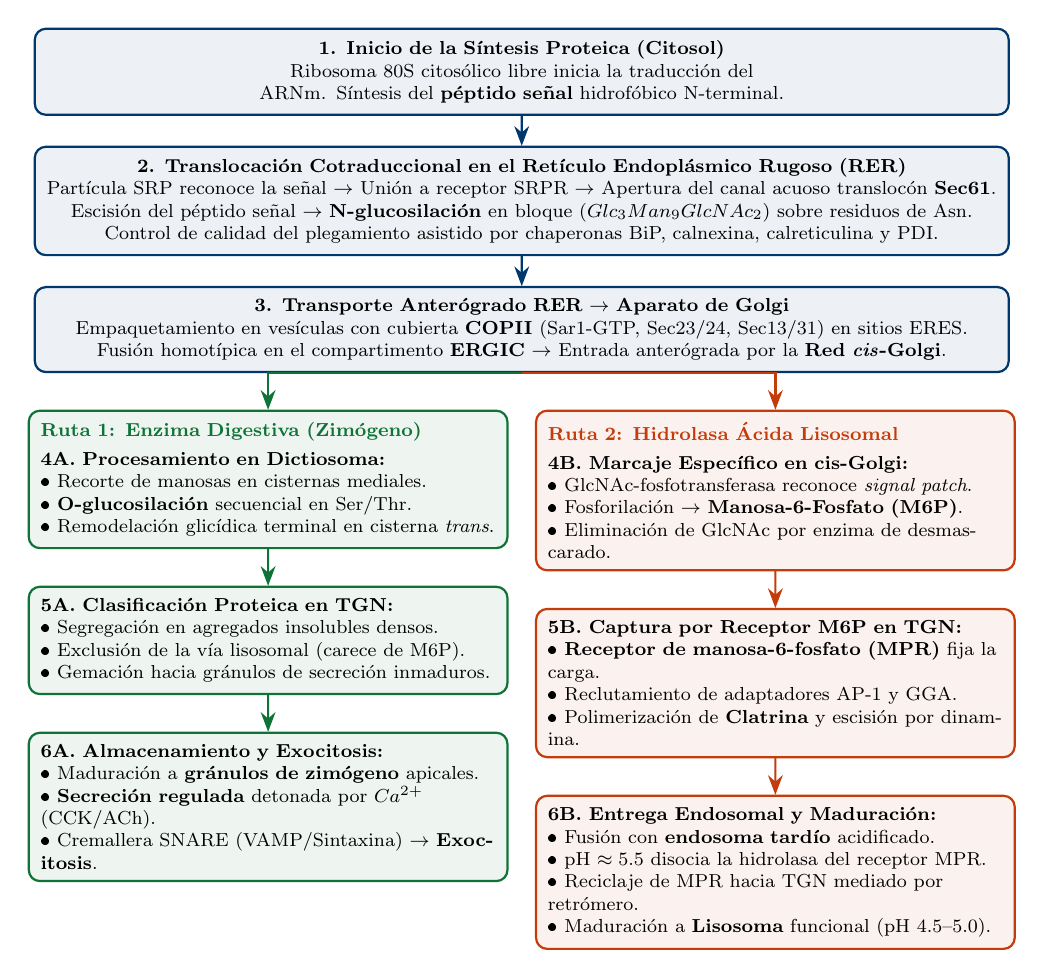
\begin{tikzpicture}[
  scale=0.85, every node/.style={transform shape},
  shared/.style={draw=uanlblue,fill=uanlblue!7,thick,rounded corners=4pt,inner sep=5pt,font=\footnotesize,align=center},
  routeA/.style={draw=proccolor,fill=proccolor!7,thick,rounded corners=4pt,inner sep=5pt,font=\footnotesize,align=left},
  routeB/.style={draw=protcolor,fill=protcolor!7,thick,rounded corners=4pt,inner sep=5pt,font=\footnotesize,align=left},
  arrow/.style={-{Stealth[length=2.5mm]},thick,uanlblue},
  arrowA/.style={-{Stealth[length=2.5mm]},thick,proccolor},
  arrowB/.style={-{Stealth[length=2.5mm]},thick,protcolor}
]

% 1. Ribosoma
\node[shared,text width=14.2cm] (n1) at (0,0) {
  \textbf{1. Inicio de la Síntesis Proteica (Citosol)}\\
  Ribosoma 80S citosólico libre inicia la traducción del ARNm. Síntesis del \textbf{péptido señal} hidrofóbico N-terminal.
};

% 2. RER
\node[shared,text width=14.2cm,below=0.45cm of n1] (n2) {
  \textbf{2. Translocación Cotraduccional en el Retículo Endoplásmico Rugoso (RER)}\\
  Partícula SRP reconoce la señal $\to$ Unión a receptor SRPR $\to$ Apertura del canal acuoso translocón \textbf{Sec61}.\\
  Escisión del péptido señal $\to$ \textbf{N-glucosilación} en bloque ($Glc_3Man_9GlcNAc_2$) sobre residuos de Asn.\\
  Control de calidad del plegamiento asistido por chaperonas BiP, calnexina, calreticulina y PDI.
};

% 3. COPII y ERGIC
\node[shared,text width=14.2cm,below=0.45cm of n2] (n3) {
  \textbf{3. Transporte Anterógrado RER $\to$ Aparato de Golgi}\\
  Empaquetamiento en vesículas con cubierta \textbf{COPII} (Sar1-GTP, Sec23/24, Sec13/31) en sitios ERES.\\
  Fusión homotípica en el compartimento \textbf{ERGIC} $\to$ Entrada anterógrada por la \textbf{Red \textit{cis}-Golgi}.
};

% 4. Bifurcacion
\coordinate (split) at ([yshift=-0.55cm]n3.south);
\node[routeA,text width=6.8cm,anchor=north east] (rA_golgi) at ([xshift=-0.2cm]split) {
  \textbf{\textcolor{proccolor}{Ruta 1: Enzima Digestiva (Zimógeno)}}\\[0.1cm]
  \textbf{4A. Procesamiento en Dictiosoma:}\\
  • Recorte de manosas en cisternas mediales.\\
  • \textbf{O-glucosilación} secuencial en Ser/Thr.\\
  • Remodelación glicídica terminal en cisterna \textit{trans}.
};

\node[routeB,text width=6.8cm,anchor=north west] (rB_golgi) at ([xshift=0.2cm]split) {
  \textbf{\textcolor{protcolor}{Ruta 2: Hidrolasa Ácida Lisosomal}}\\[0.1cm]
  \textbf{4B. Marcaje Específico en cis-Golgi:}\\
  • GlcNAc-fosfotransferasa reconoce \textit{signal patch}.\\
  • Fosforilación $\to$ \textbf{Manosa-6-Fosfato (M6P)}.\\
  • Eliminación de GlcNAc por enzima de desmascarado.
};

% 5. Clasificacion TGN
\node[routeA,text width=6.8cm,below=0.55cm of rA_golgi] (rA_tgn) {
  \textbf{5A. Clasificación Proteica en TGN:}\\
  • Segregación en agregados insolubles densos.\\
  • Exclusión de la vía lisosomal (carece de M6P).\\
  • Gemación hacia gránulos de secreción inmaduros.
};

\node[routeB,text width=6.8cm,below=0.55cm of rB_golgi] (rB_tgn) {
  \textbf{5B. Captura por Receptor M6P en TGN:}\\
  • \textbf{Receptor de manosa-6-fosfato (MPR)} fija la carga.\\
  • Reclutamiento de adaptadores AP-1 y GGA.\\
  • Polimerización de \textbf{Clatrina} y escisión por dinamina.
};

% 6. Destino Final
\node[routeA,text width=6.8cm,below=0.55cm of rA_tgn] (rA_dest) {
  \textbf{6A. Almacenamiento y Exocitosis:}\\
  • Maduración a \textbf{gránulos de zimógeno} apicales.\\
  • \textbf{Secreción regulada} detonada por $Ca^{2+}$ (CCK/ACh).\\
  • Cremallera SNARE (VAMP/Sintaxina) $\to$ \textbf{Exocitosis}.
};

\node[routeB,text width=6.8cm,below=0.55cm of rB_tgn] (rB_dest) {
  \textbf{6B. Entrega Endosomal y Maduración:}\\
  • Fusión con \textbf{endosoma tardío} acidificado.\\
  • pH $\approx 5.5$ disocia la hidrolasa del receptor MPR.\\
  • Reciclaje de MPR hacia TGN mediado por retrómero.\\
  • Maduración a \textbf{Lisosoma} funcional (pH 4.5--5.0).
};

% Conexiones
\draw[arrow] (n1) -- (n2);
\draw[arrow] (n2) -- (n3);

\draw[arrowA] (n3.south) -| (rA_golgi.north);
\draw[arrowB] (n3.south) -| (rB_golgi.north);

\draw[arrowA] (rA_golgi) -- (rA_tgn);
\draw[arrowB] (rB_golgi) -- (rB_tgn);

\draw[arrowA] (rA_tgn) -- (rA_dest);
\draw[arrowB] (rB_tgn) -- (rB_dest);

\end{tikzpicture}
\caption{Esquema II: Diagrama de flujo ultraestructural del encaminamiento proteico comparado en la célula acinar pancreática (Ruta 1: Enzima digestiva hacia exocitosis regulada vs. Ruta 2: Hidrolasa ácida hacia el lisosoma).}
\label{fig:esquema_rutas}
\end{figure}

\clearpage

\section{Parte II. Dinámica Macromolecular y Tránsito en el Sistema de Endomembranas}
Para integrar los 13 conceptos obligatorios, explico cómo se coordinan dentro del funcionamiento normal de la célula:

El recorrido de las proteínas comienza cuando el ribosoma traduce el ARN en el citoplasma. Al salir la primera parte de la cadena, llamada \textbf{péptido señal}, la célula identifica que debe entrar al retículo; el ribosoma se une a la membrana y la proteína ingresa al interior al mismo tiempo que se produce, mediante una \textbf{traducción cotraduccional} \parencite{salazar2018biologia, alberts2022molecular}. En el retículo se le transfiere un grupo de azúcares a residuos de asparagina (\textbf{N-glucosilación}), lo que ayuda a su correcto plegamiento \parencite{mathews2013bioquimica}. Después, al avanzar por el aparato de Golgi, se le agregan azúcares en residuos de serina o treonina mediante la \textbf{O-glucosilación} \parencite{karp2019biologia}.

El movimiento entre organelos se realiza con pequeñas vesículas recubiertas por proteínas: las vesículas con cubierta \textbf{COPII} transportan la carga hacia adelante desde el retículo hacia el Golgi, mientras que las vesículas con cubierta \textbf{COPI} realizan la ruta contraria para regresar al retículo las proteínas que se escaparon por error \parencite{fortoul2020histologia, lodish2021molecular}. Al llegar a la red \textit{trans}-Golgi, la célula realiza una cuidadosa \textbf{clasificación proteica} para asegurar el correcto \textbf{encaminamiento proteico} de cada proteína \parencite{alberts2022molecular}.

Las enzimas que van a degradar desechos llevan una etiqueta que es reconocida por el \textbf{receptor de manosa-6-fosfato}; este receptor jala una cubierta de \textbf{clatrina} para formar vesículas que viajan hacia los endosomas, los cuales maduran hasta convertirse en un \textbf{lisosoma} con enzimas activas a pH ácido \parencite{kierszenbaum2020histologia, lieberman2018marks}. En cambio, las enzimas digestivas que saldrán de la célula se acumulan en gránulos y solo se liberan cuando hay comida en el tracto digestivo mediante \textbf{secreción regulada}, donde la vesícula se une a la membrana celular y vacía su contenido por \textbf{exocitosis} \parencite{kierszenbaum2020histologia, karp2019biologia}.

Para entender cómo funciona el transporte y reciclaje de este receptor, en la Figura~\ref{fig:esquema_m6p} muestro el ciclo del receptor de manosa-6-fosfato:

\begin{figure}[htbp]
\centering
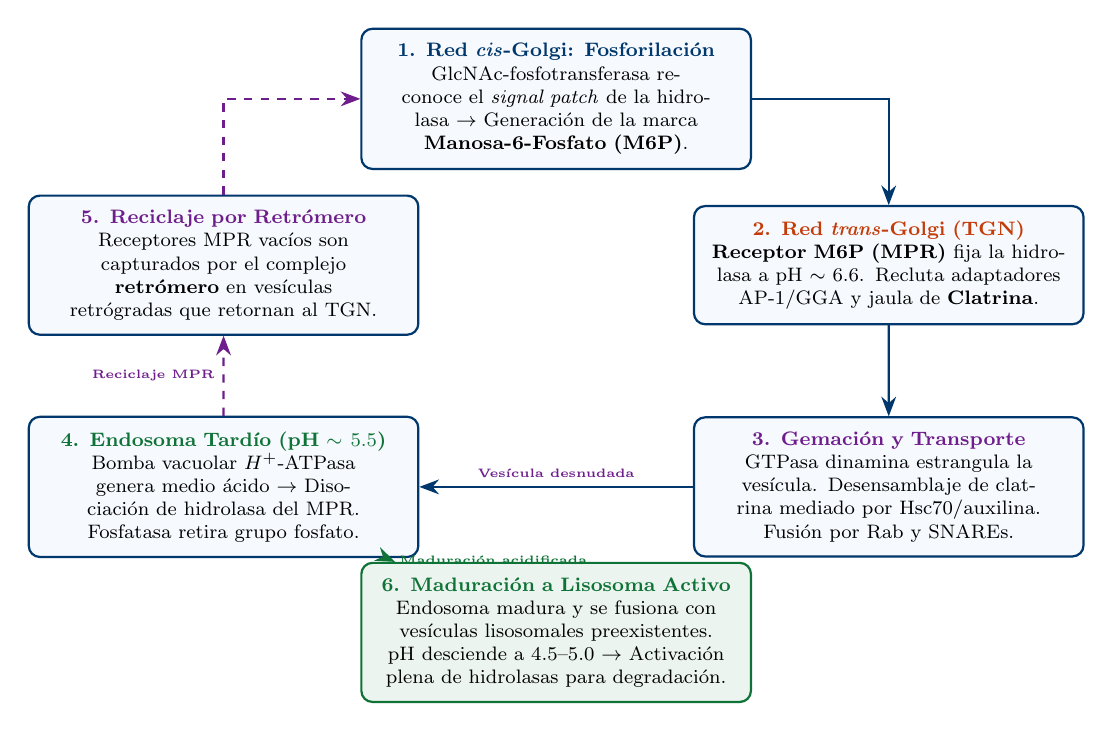
\begin{tikzpicture}[
  scale=0.88, every node/.style={transform shape},
  stepbox/.style={draw=uanlblue,fill=boxbg,thick,rounded corners=4pt,inner sep=6pt,font=\footnotesize,align=center,text width=5.2cm},
  arrow/.style={-{Stealth[length=2.5mm]},thick,uanlblue},
  retarrow/.style={-{Stealth[length=2.5mm]},thick,pathcolor,dashed}
]

% Nodos del ciclo
\node[stepbox] (s1) at (0, 3.2) {
  \textbf{\textcolor{uanlblue}{1. Red \textit{cis}-Golgi: Fosforilación}}\\
  GlcNAc-fosfotransferasa reconoce el \textit{signal patch} de la hidrolasa $\to$ Generación de la marca \textbf{Manosa-6-Fosfato (M6P)}.
};

\node[stepbox] (s2) at (4.8, 0.8) {
  \textbf{\textcolor{protcolor}{2. Red \textit{trans}-Golgi (TGN)}}\\
  \textbf{Receptor M6P (MPR)} fija la hidrolasa a pH $\sim 6.6$. Recluta adaptadores AP-1/GGA y jaula de \textbf{Clatrina}.
};

\node[stepbox] (s3) at (4.8, -2.4) {
  \textbf{\textcolor{pathcolor}{3. Gemación y Transporte}}\\
  GTPasa dinamina estrangula la vesícula. Desensamblaje de clatrina mediado por Hsc70/auxilina. Fusión por Rab y SNAREs.
};

\node[stepbox] (s4) at (-4.8, -2.4) {
  \textbf{\textcolor{proccolor}{4. Endosoma Tardío (pH $\sim 5.5$)}}\\
  Bomba vacuolar $H^+$-ATPasa genera medio ácido $\to$ Disociación de hidrolasa del MPR. Fosfatasa retira grupo fosfato.
};

\node[stepbox] (s5) at (-4.8, 0.8) {
  \textbf{\textcolor{pathcolor}{5. Reciclaje por Retrómero}}\\
  Receptores MPR vacíos son capturados por el complejo \textbf{retrómero} en vesículas retrógradas que retornan al TGN.
};

\node[stepbox,draw=proccolor,fill=proccolor!8] (s6) at (0, -4.5) {
  \textbf{\textcolor{proccolor}{6. Maduración a Lisosoma Activo}}\\
  Endosoma madura y se fusiona con vesículas lisosomales preexistentes.\\
  pH desciende a 4.5--5.0 $\to$ Activación plena de hidrolasas para degradación.
};

% Flechas del ciclo
\draw[arrow] (s1) -| (s2);
\draw[arrow] (s2) -- (s3);
\draw[arrow] (s3) -- (s4) node[midway,above,font=\tiny\bfseries,text=pathcolor] {Vesícula desnudada};
\draw[retarrow] (s4) -- (s5) node[midway,left,font=\tiny\bfseries,text=pathcolor] {Reciclaje MPR};
\draw[retarrow] (s5) |- (s1);
\draw[arrow,draw=proccolor] (s4) -- (s6) node[midway,right,font=\tiny\bfseries,text=proccolor] {Maduración acidificada};

\end{tikzpicture}
\caption{Esquema III: Ciclo molecular del receptor de manosa-6-fosfato (MPR), transporte selectivo mediado por clatrina y reciclaje por el complejo retrómero.}
\label{fig:esquema_m6p}
\end{figure}

\section{Parte III. Análisis Funcional}

\subsection{Pregunta 1: ¿Por qué el aparato de Golgi puede compararse con un centro de distribución logística?}
El aparato de Golgi funciona de manera muy similar a un centro de paquetería o distribución de mercancías por las siguientes razones:
\begin{enumerate}
    \item \textbf{Recepción de paquetes:} Al igual que un almacén central recibe camiones con mercancía que viene de la fábrica, la cara \textit{cis} de Golgi recibe las vesículas con proteínas recién hechas procedentes del retículo endoplásmico rugoso.
    \item \textbf{Línea de terminado y empaque:} Conforme las proteínas avanzan por las cisternas (\textit{cis} $\to$ mediales $\to$ \textit{trans}), distintas enzimas les dan el acabado final: les recortan azúcares, agregan nuevos grupos y aplican la O-glucosilación para que queden listas \parencite{mathews2013bioquimica, fortoul2020histologia}.
    \item \textbf{Lectura de etiquetas y clasificación:} En la red \textit{trans}-Golgi (TGN), el organelo revisa las etiquetas moleculares: si la proteína tiene manosa-6-fosfato se envía a los lisosomas; si tiene señales para la membrana se envía a la superficie celular; y si son enzimas digestivas sin marca especial, se acumulan en gránulos de secreción regulada \parencite{alberts2022molecular, lodish2021molecular}.
    \item \textbf{Envío en transporte especializado:} El Golgi empaca cada proteína en la vesícula adecuada (con clatrina para lisosomas o vesículas de secreción para salir) y les coloca señales de entrega para que lleguen exactamente al organelo correcto \parencite{karp2019biologia}.
\end{enumerate}

\subsection{Pregunta 2: Explicación de por qué el RER y el aparato de Golgi no son el destino final de muchas proteínas}
El retículo endoplásmico rugoso y el aparato de Golgi son estaciones de paso donde las proteínas se fabrican, modifican y clasifican, pero casi ninguna proteína realiza allí su trabajo final \parencite{lodish2021molecular}. Esto se debe a dos razones claras:
\begin{itemize}
    \item \textbf{Peligro de autodigestión y condiciones de trabajo:} Las enzimas digestivas deben actuar en el intestino para degradar los alimentos; si estuvieran activas dentro del retículo, digerirían las membranas de la célula y la matarían \parencite{kierszenbaum2020histologia}. De igual forma, las enzimas lisosomales necesitan un pH muy ácido (4.5 a 5.0) para activarse, mientras que el retículo y el Golgi tienen un pH casi neutro (alrededor de 7.0), por lo que no pueden funcionar ahí \parencite{lieberman2018marks}.
    \item \textbf{Mecanismo de retención activa:} Las únicas proteínas que se quedan en el retículo o en el Golgi son las que trabajan para el propio organelo (como chaperonas BiP, calreticulina y enzimas que pegan azúcares). Para quedarse, estas proteínas tienen una señal especial de retención (como la señal KDEL). Todas las demás proteínas que no tienen esta señal de retención son empacadas y continúan su viaje hacia el siguiente destino \parencite{alberts2022molecular, fortoul2020histologia}.
\end{itemize}

\subsection{Pregunta 3: ¿Qué consecuencias tendría que una hidrolasa lisosomal no recibiera la marca de manosa-6-fosfato?}
Si una hidrolasa lisosomal no recibe la marca de manosa-6-fosfato (M6P), se produce un grave problema en el transporte celular \parencite{lieberman2018marks, karp2019biologia}:
\begin{enumerate}
    \item \textbf{La enzima se sale de la célula por error:} Como la enzima no tiene la marca de manosa-6-fosfato, el receptor en la red \textit{trans}-Golgi no la reconoce. Al no ser retenida para los lisosomas, la célula la envía por la ruta por defecto hacia afuera, liberándola al torrente sanguíneo mediante secreción constitutiva \parencite{alberts2022molecular, lodish2021molecular}.
    \item \textbf{Los lisosomas se quedan vacíos:} Los lisosomas carecen de enzimas para degradar y se vuelven incapaces de digerir desechos celulares o partes viejas de la célula.
    \item \textbf{Acumulación de basura celular:} Al no poder degradarse, los lípidos y azúcares complejos se acumulan dentro de los lisosomas, hinchándolos y formando grandes cuerpos de inclusión que entorpecen el funcionamiento de la célula.
    \item \textbf{Enfermedad de células I (mucolipidosis tipo II):} En medicina, esto provoca una enfermedad genética grave llamada Enfermedad de Células de Inclusión (o células I), causada por una falla en la enzima del Golgi que pone el fosfato. Los pacientes tienen niveles muy altos de hidrolasas en la sangre pero sus células no pueden limpiar sus desechos, lo que causa graves deformidades en los huesos, retraso en el desarrollo y muerte a temprana edad \parencite{lieberman2018marks, kierszenbaum2020histologia}.
\end{enumerate}

\subsection{Pregunta 4: Relación de Cubiertas Vesiculares con su Función en el Tránsito Intracelular}
Las vesículas no se desprenden solas; necesitan que se ensamblen proteínas de cubierta en su superficie para curvar la membrana y seleccionar la carga correcta (Figura~\ref{fig:esquema_cubiertas}) \parencite{alberts2022molecular, lodish2021molecular}.

\begin{figure}[htbp]
\centering
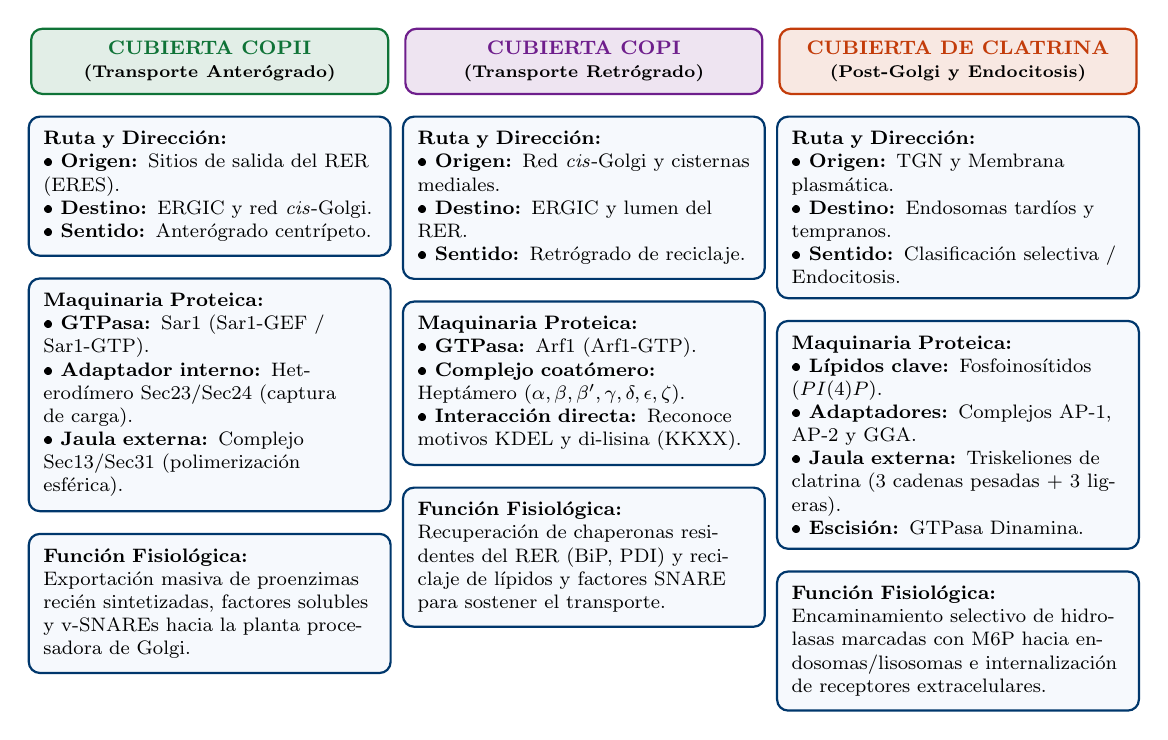
\begin{tikzpicture}[
  scale=0.88, every node/.style={transform shape},
  colbox/.style={draw=uanlblue,fill=boxbg,thick,rounded corners=4pt,inner sep=6pt,font=\footnotesize,align=left,text width=4.8cm},
  headercopii/.style={draw=proccolor,fill=proccolor!12,thick,rounded corners=4pt,inner sep=5pt,font=\bfseries\footnotesize,align=center,text width=4.8cm},
  headercopi/.style={draw=pathcolor,fill=pathcolor!12,thick,rounded corners=4pt,inner sep=5pt,font=\bfseries\footnotesize,align=center,text width=4.8cm},
  headerclat/.style={draw=protcolor,fill=protcolor!12,thick,rounded corners=4pt,inner sep=5pt,font=\bfseries\footnotesize,align=center,text width=4.8cm}
]

% Headers
\node[headercopii] (h1) at (-5.4, 3.5) {\textcolor{proccolor}{CUBIERTA COPII}\\\scriptsize (Transporte Anterógrado)};
\node[headercopi] (h2) at (0, 3.5) {\textcolor{pathcolor}{CUBIERTA COPI}\\\scriptsize (Transporte Retrógrado)};
\node[headerclat] (h3) at (5.4, 3.5) {\textcolor{protcolor}{CUBIERTA DE CLATRINA}\\\scriptsize (Post-Golgi y Endocitosis)};

% Row 1: Origen y Destino
\node[colbox,below=0.3cm of h1] (b1_1) {
  \textbf{Ruta y Dirección:}\\
  • \textbf{Origen:} Sitios de salida del RER (ERES).\\
  • \textbf{Destino:} ERGIC y red \textit{cis}-Golgi.\\
  • \textbf{Sentido:} Anterógrado centrípeto.
};
\node[colbox,below=0.3cm of h2] (b2_1) {
  \textbf{Ruta y Dirección:}\\
  • \textbf{Origen:} Red \textit{cis}-Golgi y cisternas mediales.\\
  • \textbf{Destino:} ERGIC y lumen del RER.\\
  • \textbf{Sentido:} Retrógrado de reciclaje.
};
\node[colbox,below=0.3cm of h3] (b3_1) {
  \textbf{Ruta y Dirección:}\\
  • \textbf{Origen:} TGN y Membrana plasmática.\\
  • \textbf{Destino:} Endosomas tardíos y tempranos.\\
  • \textbf{Sentido:} Clasificación selectiva / Endocitosis.
};

% Row 2: Maquinaria Molecular
\node[colbox,below=0.3cm of b1_1] (b1_2) {
  \textbf{Maquinaria Proteica:}\\
  • \textbf{GTPasa:} Sar1 (Sar1-GEF / Sar1-GTP).\\
  • \textbf{Adaptador interno:} Heterodímero Sec23/Sec24 (captura de carga).\\
  • \textbf{Jaula externa:} Complejo Sec13/Sec31 (polimerización esférica).
};
\node[colbox,below=0.3cm of b2_1] (b2_2) {
  \textbf{Maquinaria Proteica:}\\
  • \textbf{GTPasa:} Arf1 (Arf1-GTP).\\
  • \textbf{Complejo coatómero:} Heptámero $(\alpha, \beta, \beta', \gamma, \delta, \epsilon, \zeta)$.\\
  • \textbf{Interacción directa:} Reconoce motivos KDEL y di-lisina (KKXX).
};
\node[colbox,below=0.3cm of b3_1] (b3_2) {
  \textbf{Maquinaria Proteica:}\\
  • \textbf{Lípidos clave:} Fosfoinosítidos ($PI(4)P$).\\
  • \textbf{Adaptadores:} Complejos AP-1, AP-2 y GGA.\\
  • \textbf{Jaula externa:} Triskeliones de clatrina (3 cadenas pesadas + 3 ligeras).\\
  • \textbf{Escisión:} GTPasa Dinamina.
};

% Row 3: Función Biomecánica
\node[colbox,below=0.3cm of b1_2] (b1_3) {
  \textbf{Función Fisiológica:}\\
  Exportación masiva de proenzimas recién sintetizadas, factores solubles y v-SNAREs hacia la planta procesadora de Golgi.
};
\node[colbox,below=0.3cm of b2_2] (b2_3) {
  \textbf{Función Fisiológica:}\\
  Recuperación de chaperonas residentes del RER (BiP, PDI) y reciclaje de lípidos y factores SNARE para sostener el transporte.
};
\node[colbox,below=0.3cm of b3_2] (b3_3) {
  \textbf{Función Fisiológica:}\\
  Encaminamiento selectivo de hidrolasas marcadas con M6P hacia endosomas/lisosomas e internalización de receptores extracelulares.
};

\end{tikzpicture}
\caption{Esquema IV: Comparación de las cubiertas vesiculares COPII, COPI y clatrina.}
\label{fig:esquema_cubiertas}
\end{figure}

En la Tabla~\ref{tab:cubiertas_vesiculares} comparo los tres tipos de cubiertas, su origen, destino y función principal:

\begin{table}[htbp]
\centering
\scriptsize
\setlength{\tabcolsep}{4.5pt}
\renewcommand{\arraystretch}{1.08}
\begin{tabularx}{\textwidth}{p{1.6cm}p{2.8cm}p{2.8cm}Z}
\toprule
\textbf{Cubierta} & \textbf{Compartimento de Origen} & \textbf{Compartimento de Destino} & \textbf{Componentes Clave y Función Específica} \\
\midrule
\textbf{COPII} & Sitios de salida del RER (ERES). & Compartimento intermedio RE-Golgi (ERGIC) y red \textit{cis}-Golgi. & 
\textbf{GTPasa Sar1, heterodímero Sec23/Sec24 y complejo Sec13/Sec31.} Media el \textbf{transporte anterógrado} (hacia adelante): forma vesículas que sacan proteínas recién plegadas y lípidos del RER hacia el Golgi \parencite{alberts2022molecular, fortoul2020histologia}. \\
\addlinespace[0.15cm]
\textbf{COPI} & Red \textit{cis}-Golgi y cisternas mediales del dictiosoma. & Cisternas de Golgi precedentes, ERGIC y lumen del RER. & 
\textbf{GTPasa Arf1 y complejo coatómero.} Media el \textbf{transporte retrógrado} (hacia atrás): recupera enzimas y chaperonas del RER con señal KDEL que se escaparon, y recicla membranas para mantener el flujo \parencite{lodish2021molecular, fortoul2020histologia}. \\
\addlinespace[0.15cm]
\textbf{Clatrina} & Red \textit{trans}-Golgi (TGN) y membrana plasmática. & Endosomas tardíos y tempranos, lisosomas (vía indirecta). & 
\textbf{Triskeliones de clatrina, proteínas adaptadoras (AP-1, AP-2) y dinamina.} Media el \textbf{transporte post-Golgi y endocitosis}: empaca hidrolasas con señal M6P para mandarlas a los lisosomas, y ayuda a meter moléculas desde el exterior \parencite{mathews2013bioquimica, kierszenbaum2020histologia}. \\
\bottomrule
\end{tabularx}
\caption{Comparación de las cubiertas vesiculares y su función en el transporte celular.}
\label{tab:cubiertas_vesiculares}
\end{table}

\clearpage

\section{Parte IV. Integración Final}
A partir de este recorrido por cada organelo, entiendo que el sistema de endomembranas funciona como una red de transporte organizada y en una sola dirección. Cada compartimento tiene su trabajo: el RER fabrica las proteínas y vigila que queden bien dobladas; el Golgi las modifica agregando azúcares y les pone la etiqueta de destino; y la red \textit{trans}-Golgi las clasifica y empaqueta en vesículas hacia su lugar final. Todo este movimiento de vesículas, guiado por cubiertas de proteínas y receptores específicos, asegura que las enzimas lleguen a donde deben actuar sin dañar a la célula, manteniendo su funcionamiento ordenado y saludable \parencite{alberts2022molecular, lodish2021molecular, fortoul2020histologia}.

\section{Perspectiva y Relevancia Agronómica}
Como estudiante de agronomía en la Facultad de Agronomía de la UANL (Campus Escobedo), veo que aunque en clase solemos revisar estos procesos con ejemplos de células animales (como el páncreas), en las plantas cultivadas el sistema de endomembranas cumple funciones muy parecidas y de gran importancia para el campo \parencite{taiz2015plant}:
\begin{itemize}
    \item \textbf{Almacenamiento de proteínas en semillas:} En granos de leguminosas (como frijol y soya) y cereales (maíz y trigo), las proteínas de reserva que comemos se sintetizan en el RER y se mandan a través del Golgi hacia vacuolas especiales de almacenamiento. De este proceso depende directamente la calidad nutricional y el contenido de proteína de las cosechas.
    \item \textbf{Construcción de la pared celular:} En las plantas, el aparato de Golgi tiene la tarea extra de fabricar azúcares complejos (hemicelulosas y pectinas). Estos materiales salen en vesículas hacia la pared celular para darle rigidez al tallo y proteger a la planta del acame o quebrado por viento.
    \item \textbf{Defensa contra plagas y enfermedades:} Cuando un hongo o bacteria ataca una hoja, la célula vegetal dirige rápidamente vesículas cargadas de calosa y compuestos de defensa hacia el punto de entrada para levantar una barrera y frenar la infección.
\end{itemize}

\clearpage

\section{Conclusiones}

\textbf{El transporte celular tiene una sola dirección y sentido:} En esta actividad comprendí que el sistema de endomembranas no son bolsitas aisladas en el citoplasma, sino una cadena de producción continua que va hacia adelante. La separación entre organelos es vital: permite que la célula fabrique enzimas peligrosas (como las del páncreas o las hidrolasas) y las mantenga encerradas hasta llegar al lisosoma o al exterior, protegiéndose a sí misma de autodigerirse.

\textbf{Las etiquetas químicas definen a dónde va cada proteína:} Me quedó muy claro que la información del ADN no basta por sí sola para que una proteína llegue a su destino. Es necesario que el Golgi le agregue marcas químicas, como la manosa-6-fosfato. Si esta etiqueta falla, como ocurre en la enfermedad de células I, la célula se confunde y tira las enzimas al exterior en vez de mandarlas a los lisosomas, lo que demuestra la precisión con la que debe trabajar esta maquinaria.

\textbf{Importancia en mi carrera de agronomía:} Para mí como futuro ingeniero agrónomo, entender las endomembranas no es solo teoría de examen. Es la base para comprender cómo los cultivos de maíz, frijol y soya acumulan proteínas en sus semillas, cómo las plantas levantan paredes celulares firmes para no caerse con el viento y cómo responden a nivel celular cuando son atacadas por hongos o bacterias. Conocer estos procesos me ayuda a ver a los cultivos como seres vivos que responden desde su interior a las condiciones del campo.

\vspace{0.6cm}
\printbibliography[heading=bibintoc,title={Referencias Bibliográficas}]

\end{document}

